The mid point of $PB$ is
\begin{align}
\vec{M} =\frac{1}{2}(\vec{P}+\vec{B})
	= \myvec{4 \\ -2}  
\end{align}
which, from  \eqref{eq:dir-vec}, is equal to the direction vector of $OM$, where $\vec{O}$ is the origin.
\begin{align}
\because \vec{M} \equiv
	 \myvec{1 \\ -\frac{1}{2}},
	m = -\frac{1}{2}
\end{align}
which, from \eqref{eq:dir-vec},  is the desired slope.
See 
		\figref{fig:11/10/1/5}.
	\begin{figure}[H]
		\centering
 %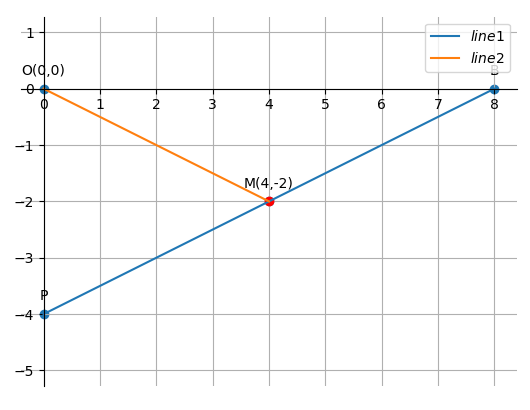
\includegraphics[width=0.75\columnwidth]{chapters/11/10/1/5/figs/line.png}
 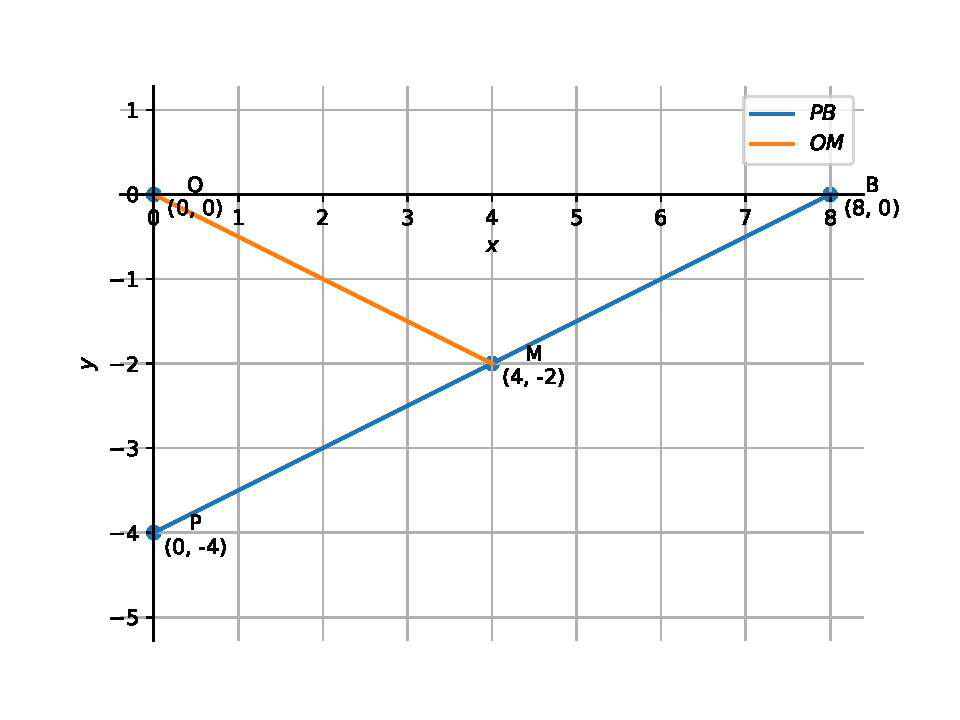
\includegraphics[width=0.75\columnwidth]{chapters/11/10/1/5/figs/fig.pdf}
		\caption{}
		\label{fig:11/10/1/5}
  	\end{figure}
